\documentclass[letter,11pt]{article}

\usepackage[spanish,es-nodecimaldot]{babel}
\usepackage[utf8]{inputenc}

\usepackage{lmodern}
\usepackage[T1]{fontenc}
\usepackage{textcomp}

\usepackage{framed}
\usepackage[svgnames]{xcolor}
\colorlet{shadecolor}{Gainsboro!50}

\usepackage{graphicx}
\usepackage{pstricks}

\usepackage{anysize}
\marginsize{3cm}{2cm}{2cm}{3cm}

\usepackage{siunitx}
\usepackage{amsmath}
\usepackage{array}

\usepackage{fancyhdr}
\usepackage{lastpage}
\pagestyle{fancy}
\fancyhf{}
\fancyhead[LE,RO]{Física Básica III}
\fancyfoot[CO,CE]{\thepage\ de \pageref{LastPage}}

\special{papersize=215.9mm,279.4mm}

\usepackage[
    pdfauthor={Carlos Eduardo Caballero Burgoa},%
    pdftitle={Física Básica III},%
    pdfsubject={Examen Final},%
    colorlinks,%
    citecolor=black,%
    filecolor=black,%
    linkcolor=black,%
    urlcolor=black,
    breaklinks]{hyperref}
\usepackage{breakurl}

\newcommand{\blankpage}{
\newpage
\thispagestyle{empty}
\mbox{}
\newpage
}

\renewcommand{\arraystretch}{1.2}

\begin{document}

\begin{center}
    {\Large \bf{Examen final}}
\end{center}

\noindent\fbox{%
    \parbox{\textwidth}{%
        Estudiante: CABALLERO BURGOA, Carlos Eduardo \\
        Carrera: Ingeniería Electromecánica \\
        Correo: cijkb.j@gmail.com
    }%
}

\vspace{0.5cm}

\begin{enumerate}
\item Dos pequeñas esferas de masa $m = 10 [g]$ están suspendidas de un punto
común mediante cuerdas de longitud $L = 50 [cm]$. Cuando cada una de las esferas
contiene la carga $q$, cada cuerda forma un ángulo $\theta$ con la vertical.
Calcular la carga $q$.

\begin{figure}[!h]
\centering
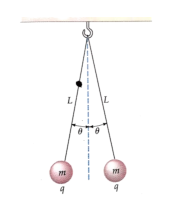
\includegraphics[scale=2.20]{resources/q1.eps}
\end{figure}

\begin{itemize}
    \item $0.24 [\mu C]$.
    \item $0.29 [\mu C]$.
    \item $0.32 [\mu C]$.
    \item $0.38 [\mu C]$.
\end{itemize}

Solución: \\

\item Un cuadripolo consta de dos dipolos próximos entre sí. La carga efectiva
en el origen es $-2q$ y las otras cargas sobre el eje ``y'' en $y = a$ e
$y = -a$ tienen valores de $q$. Tomando los valores $q = 1 [\mu C]$ y
$a = 1 [cm]$, hallar el valor del campo eléctrico en un punto sobre el eje $x$ a
gran distancia de manera que $x >> a$.

\begin{figure}[!h]
\centering
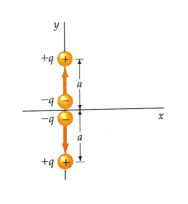
\includegraphics[scale=2.20]{resources/q2.eps}
\end{figure}

\begin{itemize}
    \item $ 2.7/x$.
    \item $-2.7/x^2$.
    \item $ 2.7/x^3$.
    \item $-2.7/x^4$.
\end{itemize}

Solución: \\

\item Una esfera uniformemente cargada de radio $R =20 [cm]$ está centrada en el
origen con una carga $Q = 2 [mC]$. Determinar la fuerza resultante que actúa
sobre una línea uniformemente cargada, orientada radialmente y con una carga
total $q = 3 [\mu C]$ con sus extremos en $x = R$ y $x = R + d$, donde
$d = 10 [cm]$.

\begin{itemize}
    \item $1350 [N]$.
    \item $ 900 [N]$.
    \item $ 864 [N]$.
    \item $ 600 [N]$.
\end{itemize}

Solución: \\

\item Una carga lineal semi-infinita de densidad uniforme
$\lambda = \num{1e-6} [C/m]$ está sobre el eje $x$ desde $x = 0$ hasta
$x = \infty$. Hallar la magnitud del campo eléctrico en el punto $x = 0 [m]$,
$y = 1 [m]$, en números enteros.

\begin{itemize}
    \item $12728 [N/C]$.
    \item $10523 [N/C]$.
    \item $ 8645 [N/C]$.
    \item $ 6019 [N/C]$.
\end{itemize}

Solución: \\

\item Cuatro cargas iguales $Q = 1 [\mu C]$ se encuentran en los vértices de un
cuadrado de lado $L = 10 [cm]$. Las cargas se dejan en libertad de una en una
siguiendo el sentido de las agujas del reloj alrededor del cuadrado. Se deja que
cada carga alcance su velocidad final a una gran distancia del cuadrado antes de
liberar la siguiente carga. Calcular la energía cinética final de la primera
carga liberada.

\begin{itemize}
    \item $487.28 [mJ]$.
    \item $243.64 [mJ]$.
    \item $153.64 [mJ]$.
    \item $ 90    [mJ]$.
\end{itemize}

Solución: \\

\item Una partícula de masa $m = \num{1e-9} [kg]$ y carga $Q = 1 [\mu C]$ está
localizada sobre el eje $x$ en $x = a$ ($a = 50 [cm]$), mientras que una segunda
partícula de igual masa y carga $-Q$ está localizada sobre el eje $x$ en
$x = -a$. Ambas se dejan en libertad en el tiempo $t = 0$. Calcular la magnitud
de la velocidad de la partícula cargada positivamente en $x = a/2$.

\begin{itemize}
    \item $6000 [m/s]$.
    \item $5000 [m/s]$.
    \item $4000 [m/s]$.
    \item $3000 [m/s]$.
\end{itemize}

Solución: \\

\item Dos condensadores idénticos de placas paralelas de $10 [\mu F]$ (cada uno)
reciben cargas iguales de $100 [\mu C]$ cada uno y luego se separan de la fuente
de carga. Mediante un cable se conectan sus placas positivas y mediante otro sus
placas negativas. Calcular la energía final almacenada en el sistema.

\begin{itemize}
    \item $1000    [\mu J]$.
    \item $ 832.64 [\mu J]$.
    \item $ 616.09 [\mu J]$.
    \item $ 476.19 [\mu J]$.
\end{itemize}

Solución: \\

\item Un condensador está formado por dos cilindros concéntricos de radios
$a = 2 [mm]$ y $b = 4 [mm]$, siendo su longitud $L = 10 [m]$. El cilindro
interior posee una carga $Q =1 [\mu C]$ y el cilindro exterior una carga $-Q$.
La región comprendida entre los cilindros está llena con un dieléctrico de
constante $k = 3$. Si el dieléctrico se desplaza (sin fricción), calcule la
energía que se necesita para extraer el dieléctrico.

\begin{itemize}
    \item $352,23 [\mu J]$.
    \item $394.37 [\mu J]$.
    \item $415.89 [\mu J]$.
    \item $448.62 [\mu J]$.
\end{itemize}

Solución: \\

\item El espacio comprendido entre dos cilindros metálicos metálicos coaxiales
de longitud $L = 50 [cm]$ y radios: $a = 1.5 [cm]$ y $b = 2.5 [cm]$ se llena
totalmente de un material de resistividad igual a $30 [\Omega m]$. Determinar la
intensidad de corriente entre los dos cilindros si se aplica una diferencia de
potencial de $10 [V]$ entre éstos.

\begin{itemize}
    \item $2.05 [A]$.
    \item $1.69 [A]$.
    \item $1.28 [A]$.
    \item $1.03 [A]$.
\end{itemize}

Solución: \\

\item Un disco no conductor de masa $M$ y radio $R = 10 [cm]$ tiene una densidad
de carga superficial uniforme de $6 [\mu C/m^2]$ y gira con una velocidad
angular de $360 [rpm]$ alrededor de su eje. Calcular el momento magnético de la
carga total del disco.

\begin{itemize}
    \item $45.24 [pA m^2]$.
    \item $41.08 [pA m^2]$.
    \item $38.45 [pA m^2]$.
    \item $33.33 [pA m^2]$.
\end{itemize}

Solución: \\

\end{enumerate}

\end{document}

